\documentclass{article}
\usepackage{geometry}
\usepackage{graphicx}
\usepackage{booktabs}
\usepackage{float}
\usepackage{array}
\usepackage{hyperref}
\usepackage[super,sort&compress]{cite}

\hypersetup{
    colorlinks=true,
    linkcolor=black,
    citecolor=black,
    urlcolor=blue
}
\newcolumntype{C}{>{\centering\arraybackslash}c}
\title{Sea Weather Station}
\author{Vasileios Zoidis, Iasonas Lamprinidis, Ioannis, Michalainas, Savvas Tzanetis}
\date{May 2025}

\begin{document}

\maketitle
\begin{center}
  \textbf{Repository:} \\
  \href{https://github.com/ioannisam/SeaWeatherStation}{github.com/ioannisam/SeaWeatherStation}
\end{center}
\bigskip
\begin{abstract}
    A brief overview of the Sea Weather Station project: goals, key features, and overall system architecture.
\end{abstract}
\tableofcontents
\clearpage

\newgeometry{top=1.5cm, bottom=1.5cm, right=1.5cm, left=1.5cm}
\section{Introduction}
This project implements a \textit{remote weather station}. The premise is to use multiple Arduino devices to create a network of data nodes. These nodes will monitor temperature, pressure and estimated wave shore impact/height at sea level. Collected data will then be displayed in a web application, to be used by fishermen, researchers or hobbyists.
    
    \subsection{Motivation and Objectives}
    
    \subsection{Report Structure}
    This report's structure mimics the workflow of our app. We will be explaining from the bottom up the architecture, design choices and development stages of our project.

    \begin{figure} [h]
        \centering
        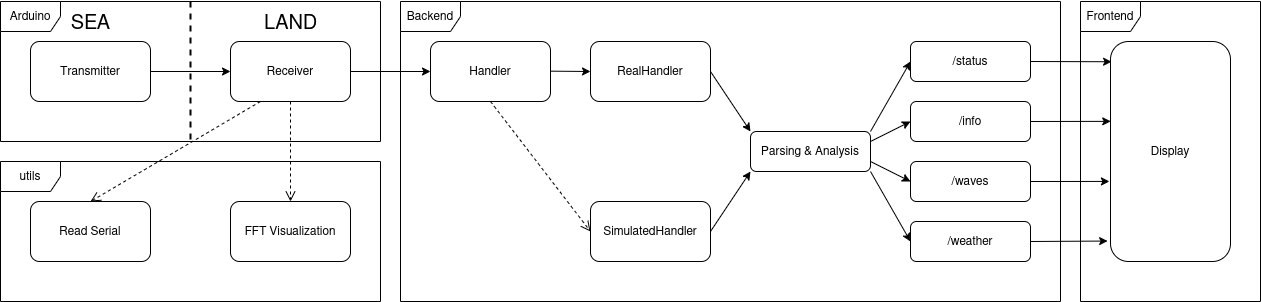
\includegraphics[width=1\linewidth]{assets/workflow.png}
        \caption{Workflow}
        \label{fig:enter-label}
    \end{figure}
    
\section{Arduino}
\subsection{Hardware Components}
    \subsubsection{Sensor Selection}
    \subsubsection{Wiring and Pinout}
    \subsubsection{Enclosure and Mounting}
\subsection{Transmitter Module}
    \subsubsection{Data Acquisition Loop}
    \subsubsection{Transmission}
    \subsubsection{Power Management}
\subsection{Receiver Module}
    \subsubsection{Reception}
    \subsubsection{Serial Output}

\section{Backend}
In this section we discuss the backend's features and capabilities, as well as its architecture. The role of the backend is to capture raw data from the sensor, analyze it, package it and send it to the frontend to be displayed in a meaningful way.

\subsection{Data Ingestion}
The data ingestion system is designed with a flexible architecture that accommodates both development and production environments through two specialized handlers; \texttt{SimulatedHandler} and \texttt{RealHandler}. Both handlers expose a consistent interface through the \texttt{SerialHandler} facade, which transparently selects the appropriate implementation based on the configured operational mode (\texttt{DEMO} or \texttt{DEPLOY}). This design pattern enables the application to operate identically regardless of data source, facilitating a smooth transition between development and production environments.

    \subsubsection{Simulated Handler}
    The \texttt{SimulatedHandler} provides a simulation environment for development and testing purposes. It generates realistic sensor data that mimics actual hardware outputs. The simulation incorporates deliberate variability -employing sinusoidal patterns with randomized amplitude, frequency and noise components- to realistically model sensor behavior. Data generation occurs in a dedicated thread running at 100Hz, maintaining a rolling buffer of 500 samples (equivalent to 5 seconds of historical acceleration data). This approach enabled us to test data processing pipelines, visualization systems and analytical algorithms without requiring physical sensor hardware.
    
    \subsubsection{Real Handler}
    The \texttt{RealHandler} establishes and maintains communication with physical Arduino-based sensor hardware via serial connection. It implements several resilience features including connection retry logic with exponential backoff, error handling for disconnection scenarios and automatic reconnection attempts. The handler continuously reads and parses incoming serial data through a dedicated thread, transforming raw string input into structured data objects according to the expected protocol format. Invalid or corrupted data is filtered through parsing logic that validates ranges and formats. Similar to its simulated counterpart, this handler maintains a time-series buffer of recent acceleration readings, enabling applications to analyze trends and patterns in the most recent sensor data.
    
    \begin{figure} [h]
        \centering
        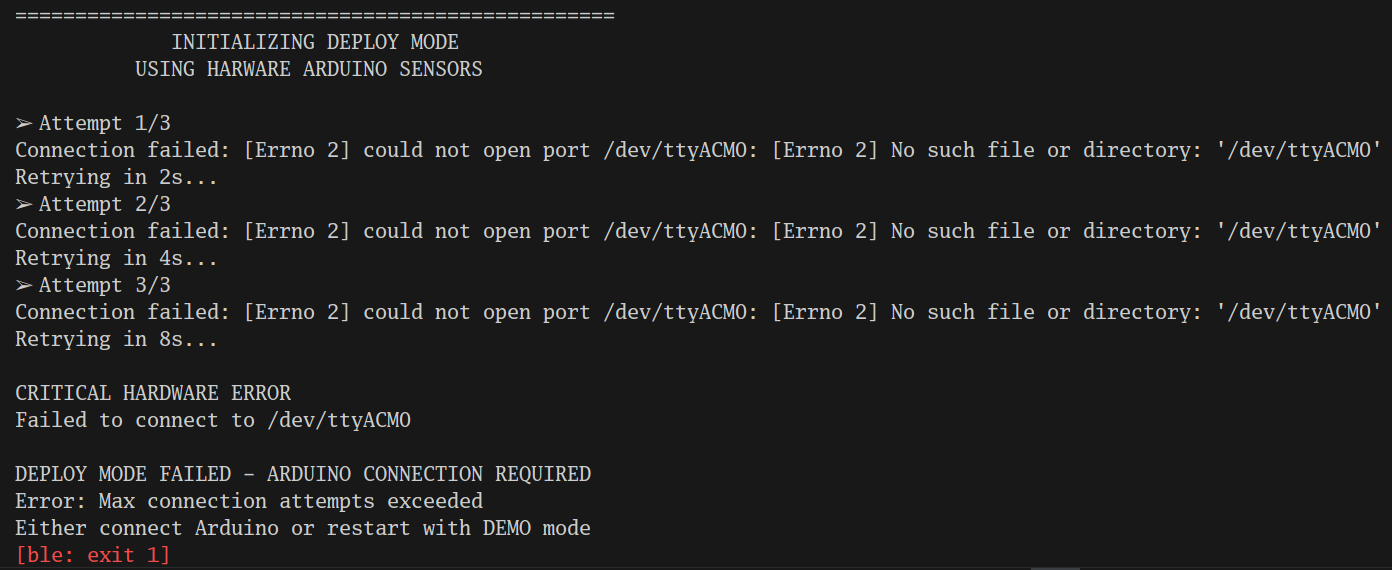
\includegraphics[width=0.75\linewidth]{assets/RealHandler.png}
        \caption{RealHandler Resilience}
        \label{fig:enter-label}
    \end{figure}

\subsection{Data Processing}

    \subsubsection{Wave Analysis}
    The wave analysis module implements a frequency-domain approach to extract meaningful metrics from raw accelerometer data. It performs Fast Fourier Transform (FFT) to identify the dominant wave frequency, filtering out low-frequency components (below 0.1 Hz) to eliminate sensor drift and environmental noise. The system converts raw accelerometer readings from LSB units to standard m/s² using a calibration factor derived from the MPU6050 sensor's sensitivity at ±2g range (datasheet). A physics-based heuristic transforms the acceleration variance into estimated wave height by applying appropriate scaling based on wave frequency, yielding actionable metrics that describe sea state conditions. The module provides a clean interface that handles edge cases such as insufficient data points and returns normalized, rounded values suitable for downstream processing.

    \subsubsection{Mathematical Background}
    The shore impact analysis implements established coastal engineering models to translate wave metrics into practical inundation forecasts \cite{stockdon2006}. The system calculates fundamental wave parameters including period (reciprocal of frequency) and deep-water wavelength using standard gravity-based equations. The core of the analysis employs the Iribarren number (surf similarity parameter) to classify wave behavior as either dissipative or reflective/intermediate, applying the appropriate runup estimation formula for each regime. The model classifies hazard zones based on runup thresholds, with values exceeding 0.9 meters designated as high-risk (VE zone) \cite{fema2022}. The final inundation distance is calculated by applying the slope correction factor, providing horizontal reach estimates critical for coastal planning.

\subsection{API Endpoints}
In this section we analyze the API endpoints available for the frontend to call

    \subsubsection{Status}
    The /status endpoint provides essential system telemetry for monitoring the operational state of the device. It returns a JSON payload containing connectivity status, power information (battery percentage), and geolocation coordinates derived from the sensor data stream. The endpoint also includes signal strength metrics (measured in dBm) to facilitate deployment troubleshooting and network quality assessment. By serving as a lightweight health check, this endpoint enables rapid verification of device functionality without interrogating the more resource-intensive data processing pipelines.

    \subsubsection{Info}
    The /info endpoint exposes environmental context data captured by the sensor array, specifically temperature (in degrees Celsius) and barometric pressure (in hectopascals).

    \subsubsection{Waves}
    The /waves endpoint delivers processed wave characteristics and their projected coastal impact. It retrieves the acceleration time-series buffer from the sensor handler and passes it through the wave analysis pipeline to extract frequency and height parameters. These metrics are then fed into the shore impact model to calculate vertical runup height, FEMA flood zone classification, and horizontal inundation distance based on a predefined slope parameter (set to 0.05 const). This endpoint represents the system's primary analytical output, transforming raw sensor data into actionable coastal flooding information delivered in a standardized JSON format.

    \subsubsection{Weather}
    The /weather endpoint enriches the system's data with third-party meteorological information by interfacing with the OpenWeatherMap API. It dynamically constructs API requests using the device's current geolocation coordinates and securely transmits the authentication key from environment variables. The endpoint parses the response to extract wind parameters (speed and direction) along with general weather conditions and human-readable descriptions.

\subsection{Test Functions and Utilities}
    \subsubsection{Package Check}
    The package check utility verifies that all dependencies meet the required version specifications, preventing compatibility issues. It generates a formatted tabular output with clear visual indicators for each package's status: successfully meeting requirements (✅), outdated versions requiring updates (❌ Too Old), or missing packages that need installation (❌ Not Found).
    
    \begin{figure} [h]
        \centering
        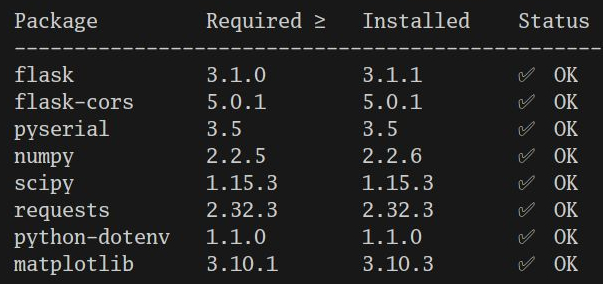
\includegraphics[width=0.5\linewidth]{assets/check-packages.png}
        \caption{Package Check}
        \label{fig:enter-label}
    \end{figure}
    
    \subsubsection{Serial Screening}
    The serial screening utility provides direct access to the raw data stream from connected Arduino hardware, bypassing the application's processing pipelines. It establishes a serial connection to the configured port using the same parameters as the main application (9600 baud) and continuously reads, parses and displays each data frame in real-time. This tool was particularly useful during initial deployment to confirm proper hardware operation before launching the complete application stack.

    \subsubsection{FFT Visualization}
    The FFT visualization tool enables detailed analysis of sensor data characteristics through both time and frequency domain representations. It captures a configurable duration of acceleration data (default 30 seconds) using the same SerialHandler interface as the main application, ensuring consistency between visualization and production operation. The tool produces a dual-panel plot showing raw acceleration values (in m/s²) against time in the upper panel and the corresponding frequency spectrum via Fast Fourier Transform in the lower panel. The visualization highlights the detected dominant frequency with a vertical marker. This dual representation allowed us to correlate time-domain patterns with their frequency components, aiding in algorithm refinement and system tuning.

    \begin{figure} [h]
        \centering
        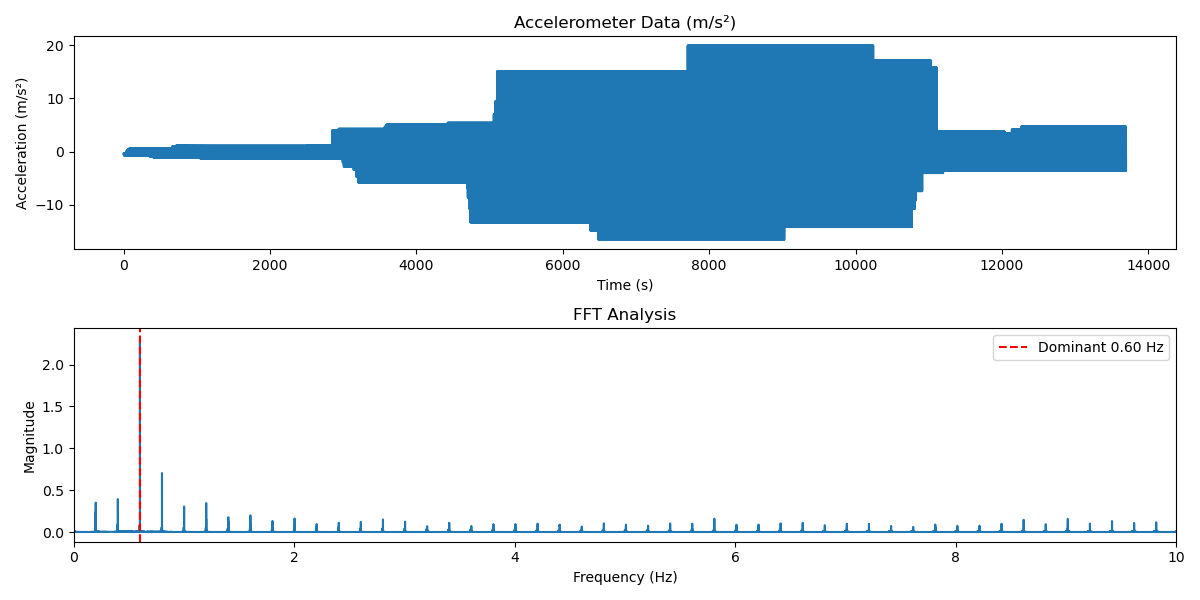
\includegraphics[width=1\linewidth]{assets/fft_visualization.png}
        \caption{FFT Visualization}
        \label{fig:enter-label}
    \end{figure}

    \subsubsection{Cleaning}
    The cleaning utility implements system maintenance functionality through a shell script that removes Python cache files. This utility improves development workflow by preventing stale bytecode from causing unexpected behavior after code changes, particularly when performing major refactoring.

\section{Frontend}
\subsection{User Interface Design}
    \subsubsection{Wireframes and Mockups}
    \subsubsection{Look and Feel}
\subsection{Data Visualization}
    \subsubsection{API Integration}
    \subsubsection{Real-time Data Flow}
    \subsubsection{Real-time Charts and Graphs}
\subsection{User Interactions}
\subsection{Testing and Accessibility}
    \subsubsection{Cross-browser Compatibility}

\section{Conclusions}
    \subsection{Summary of Achievements}
    
    \subsection{Lessons Learned}
    \subsection{Future Work}
    Future work includes:
    \begin{itemize}
        \item use solar or aeolian power to charge the battery
        \item proper battery level implementation for the /status endpoint
        \item adding more sensors
        \item 
    \end{itemize}

\appendix

\section{User Manual}
How to operate our Weather Station:
\begin{enumerate}
  \item 
  \item 
  \item 
  \item 
\end{enumerate}

\section{Bill of Materials}

\renewcommand{\arraystretch}{1.3}
\begin{table}[H]
    \centering
    \begin{tabular}{@{} C C C @{}}
        \toprule
        \multicolumn{1}{c}{\textbf{Item}} 
            & \multicolumn{1}{c}{\textbf{Quantity}} 
            & \multicolumn{1}{c}{\textbf{Price (€)}} \\
        \midrule
        Arduino Uno R3           & 1 & A \\
        DHT22 Temperature Sensor & 2 & B \\
        BMP280 Pressure Sensor   & 1 & C \\
        ESP8266 Wi-Fi Module     & 1 & D \\
        Jumper Wires (pack)      & 1 & E \\
        USB Power Cable          & 1 & F \\
        \midrule
        \textbf{Total}           &   & \textbf{G} \\
        \bottomrule
    \end{tabular}
    \caption{Bill of Materials}
    \label{tab:bom}
\end{table}

\section{Tools and Frameworks}
The following tools and frameworks were used:
\begin{itemize}
  \item Arduino IDE (Sensor Interaction)
  \item Python with Flask (Backend API)
  \item TypeScript with React (Frontend UI)
\end{itemize}

\begin{thebibliography}{9}
    \bibitem[\href{https://data-ww3.ifremer.fr/BIB/Stockdon_etal_CE2006.pdf}{1}]{stockdon2006}
        Stockdon, H.~F.; Holman, R.~A.; Reichmuth, A.; Van Ormondt, M.  
        Estimation of shoreline position and change using airborne LiDAR data.  
    \emph{Coastal Engineering} \textbf{53}(3), 2006.
    \bibitem[\href{https://www.fema.gov/sites/default/files/documents/fema_coastal-floodplain-mapping_112022.pdf}{2}]{fema2022}
        Federal Emergency Management Agency (FEMA).  
        Coastal Floodplain Mapping Report. November 2022.
\end{thebibliography}

\end{document}